The purpose of this chapter is to benchmark and evaluate memcached performance. Firstly, we will examine performance under default configuration of both the server and the client. Secondly, threading will be explored in relation to latency and throughput. Thirdly, the effect of memcached's \texttt{group size} will be explored in relation to performance. Additionally, configuration of receive and transmit queues will be explored and finally, an execution model of multiple processes will be visited in order to establish a comparison baseline. Throughout the benchmarks, we will be focusing cache performance which meets desired the QoS.


\section{Out of the Box Performance}

Firstly, we consider Memcached in it's default configuration. A list of the configuration parameters as well as the default values is presented in Section \ref{sec:memcached_configuration}. The purpose of benchmarking Memcached in the default configuration is to obtain a baseline performance. This will in turn allow us to consider potential optimizations with respect to the baseline.

The Memcached server is started with the following command.

\begin{lstlisting}
memcached -d -p 11120 -m 6144
\end{lstlisting}

We run Memcached in daemon mode (\textit{-d}), set the maximum amount of memory Memcached can use to 6GB (\textit{-m}) and finally we bind Memcached to port 11120 (textit{-p}). Note that by default, Memcached runs with 4 threads.


In order to generate a workload with increasing intensity, the number of simultaneous connections is increased linearly. As the number of connections grows, so does the number of requests per second issued to Memcached. We configure the Memtier benchmark as follows:

\begin{lstlisting}
  memtier -s <server> -p 11120 -c <connections> -t 3
    --random-data
    --key-minimum=1
    --key-maximum=100000
    --data-size=32
\end{lstlisting}
Memtier is run simultaneously on 7 hosts (distinct from the server). The Memcached server and port number are provided (\textit{-s}, \textit{-p}). Each host executing Memtier runs 3 distinct threads with \textit{c} connections in each thread. The number of connections increases linearly from 1 connection to 17 connections. As a result, the number of connections in consecutive benchmarks increases by 21. This is the result of running Memtier on 7 hosts with 3 threads per each host. Additionally, the \textit{key-minimum}, \textit{key-maximum} defines the key range utilized in this benchmark. and \textit{data-size} configuration parameters are provided for clarity and are set to the default values configured by Memtier. The result of the above configuration is to generate a linearly increasing load on the Memcached server.


\subsection{Latency, Throughput and Number of Connections}

Firstly, we are interested in the relationship between throughput and latency shown in Figure \ref{fig:memcached-default-latency-vs-ops}. Latency, both mean and 99th percentile, are plotted on the left vertical axis, the number of operations per second is plotted on the right vertical axis and the number of connections used is on the horizontal axis.

\begin{figure}[h]
    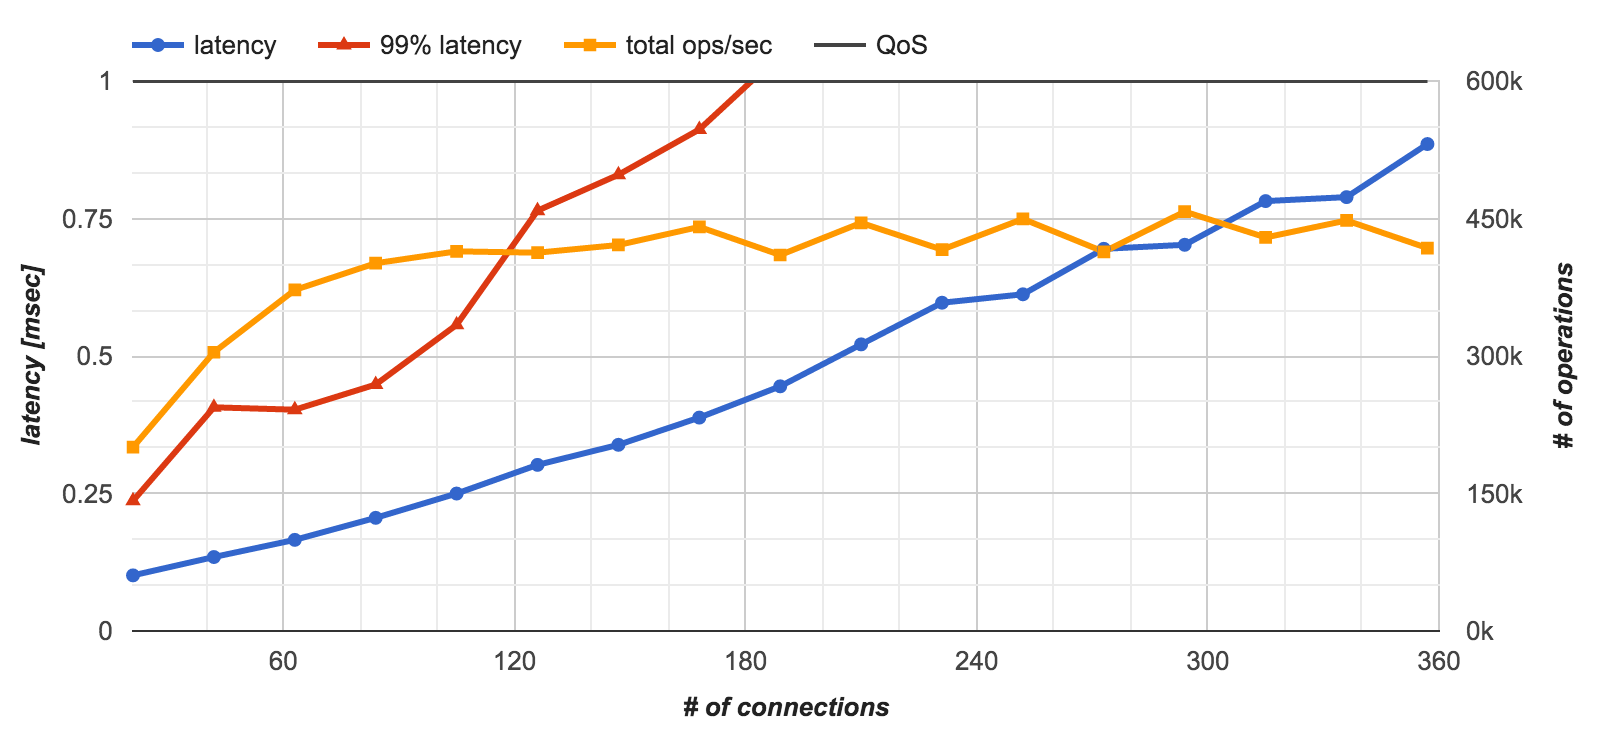
\includegraphics[width=\textwidth]{./res2/m_baseline_latency.png}
    \caption{Latency \& Throughput vs Number of Connections}
    \label{fig:memcached-default-latency-vs-ops}
\end{figure}

As the number of connections increases, mean latency increases too. There is a linear trend between the number of connections and the mean latency. The 99th percentile latency also increases with the number of connections, however, it grows faster than than the number of connections does and exceeds the required QoS constraint at 189 simultaneous connections. The total number of operations, increases quickly as the number of connections increases and begins to flatten at 100 connections or 400k requests per second. As the number of connections increases beyond 100, the throughput remains relatively stable at around 420k requests per second.

Examining the relationship between latency and throughput, we can observe that initially we are able to increase throughput to 415k requests per second, however, a further increase in throughput comes at a disproportionately larger cost in terms of 99th percentile latency. This is reasonable as there is a limit to the number of requests we can process per second, a larger number of requests will incur queuing delay which translates to increased latency.

\subsection{CPU Utilization}

Secondly, we consider the effect of the workload on the Memcached server in terms of CPU Utilization. The CPU utilization is monitored through the \textit{mpstat} \cite{mpstat} utility which reports the percentage of CPU utilization broken down into multiple categories. The following table \cite{mpstat} summarizes the responsibilities of each category.

\begin{enumerate}
    \item [\%usr] Show the percentage of CPU utilization that occurred while executing at the user level (application).
    \item [\%sys] Show the percentage of CPU utilization that occurred while executing at the system level (kernel). Note that this does not include time spent servicing hardware and software interrupts.
    \item [\%iowait] Show the percentage of time that the CPU or CPUs were idle during which the system had an outstanding disk I/O request.
    \item [\%irq] Show the percentage of time spent by the CPU or CPUs to service hardware interrupts.
    \item [\%soft] Show the percentage of time spent by the CPU or CPUs to service software interrupts.
    \item [\%idle] Show the percentage of time that the CPU or CPUs were idle and the system did not have an outstanding disk I/O request.
\end{enumerate}

For the context of this paper, \textit{\%usr} corresponds directly to the CPU utilization used by Memcached as it is the only application running on the server.

Furthermore, \textit{\%soft} represents the software interrupt issued by \textit{libevent} when a new file descriptor is available for processing, that is, a new request is available to be processed or a response is ready to be handed over to the network stack.

\begin{figure}[h]
    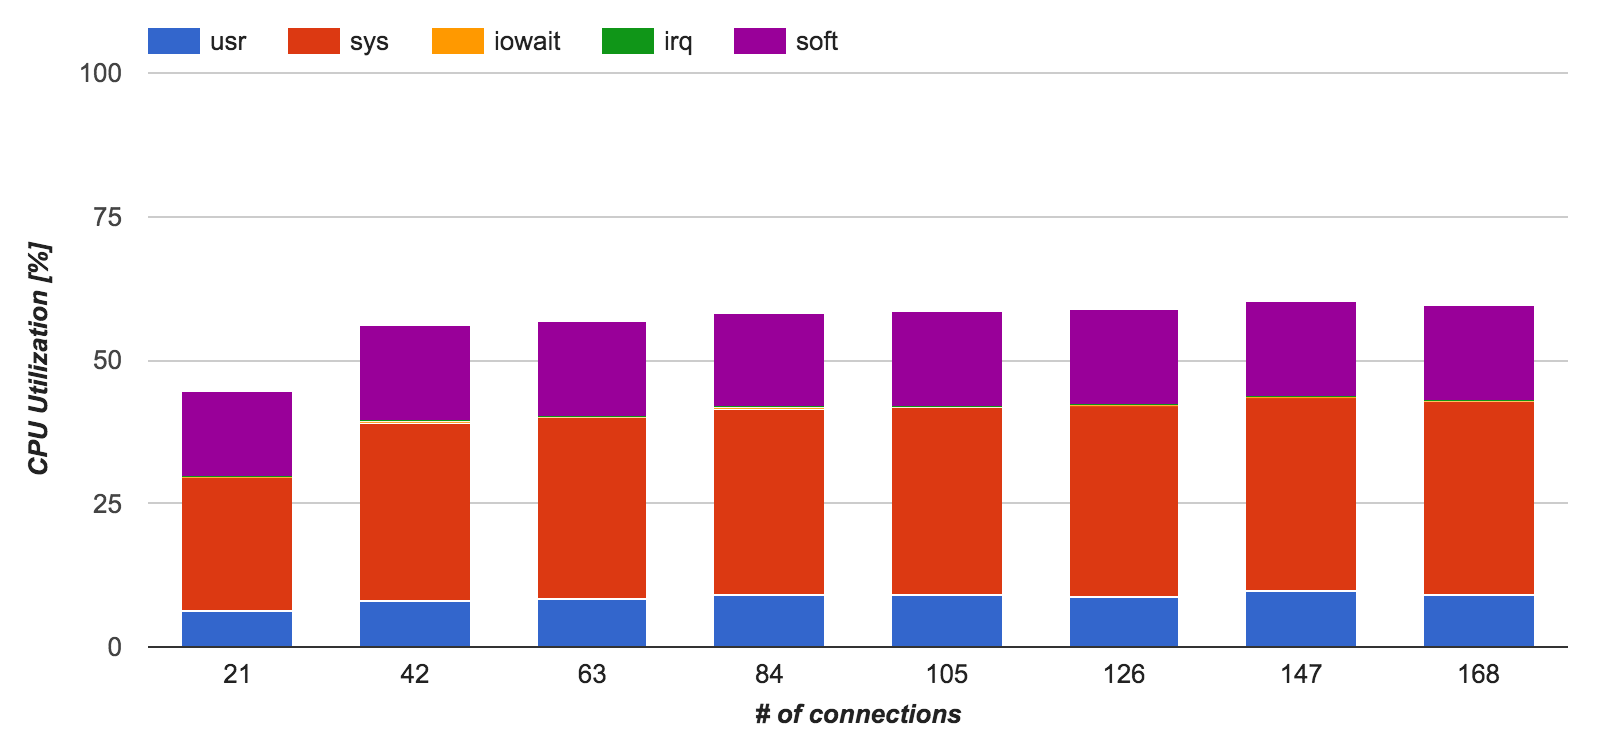
\includegraphics[width=\textwidth]{./res2/m_baseline_cpu.png}
    \caption{CPU Utilization for Out of the Box Configuration of Memcached}
    \label{fig:m_baseline_cpu}
\end{figure}

Figure \ref{fig:m_baseline_cpu} outlines the CPU Utilization broken down into mpstat categories. Note that \textit{idle} percentage is represented in the chart as the remaining transparent area of each column.

Firstly, as the number of connections increases, the \textit{usr} utilization remains nearly constant at 9\%.

Secondly, \textit{sys} utilization increases as the number of connection increases between 21 and 120 connections and remains relatively stable as the number connections increases further. This behavior corresponds to the saturation point also observed in the relationship of connections and throughput.

Thirdly, \textit{soft}, increases as the number of connections increase due to the increased number of requests per second which are required to be serviced.

Furthermore, \textit{idle}, represented as the remaining CPU utilization in each column, decreases as the number of connection increases. This is primarily due to an increase in \textit{sys} and \textit{soft}. The peak total CPU utilization is 75\%, this corresponds to 4 Memcached threads on distinct cores being utilized at 100\% and additional low utilization on the remaining 2 cores.

Finally, \textit{iowait} and \textit{irq} account for less than 0.01\% of the total CPU utilization. This is a reasonable result as Memcached is an in-memory object cache and therefore we do not expect to see any disk I/O.

As a result of the breakdown, we can conclude that Memcached itself is not CPU intensive. Rather, the bulk of the CPU utilization is taken up by the kernel as well as processing software interrupts from high number of requests per second. The overall Memcached performance appears to be tightly linked to the performance of the network stack as well as the underlying kernel. This observation is consistent with findings in MICA \cite{lim2014mica}.

Memcached performs reasonably well `out of the box', delivering 420k requests per second with 99th percentile latency meeting the QoS. The CPU utilization is dominated by the kernel and the network stack. However, Memcached has a lot to offer in terms of configuration and performance improvements which we will explore in subsequent sections.


% ________________________________________________________

\section{Memcached Thread Scalability}
Memcached, as a high performance object cache, is designed to be executed on a multi-core architecture. It implements scalability through the use multiple threads allowing memcached to utilize many core architectures. Therefore, the next step in scaling a memcached deployment is to examine the impact threads have on Memcached's performance.

Memcached execution model is capable of processing incoming and outgoing requests in parallel, however, operations executed require a global application lock to be acquired. Therefore, the expected number of threads which maximizes throughput and minimizes latency can be expected to be achieved when memcached is provisioned with the same number of threads as hardware CPU cores which is also suggested by Leverich and Kozyrakis \cite{leverich2014reconciling}.

Utilizing results from the previous section, we configure the workload with 168 connections. At this workload, we have been able to achieve a throughput of 430k requests per second with latency meeting the QoS. Therefore, the configuration for the clients is as follows:

Utilizing findings from the previous section, a configuration with 84 connections can be used to generate a consistent load while the number of threads provisioned for memcached can be varied. Therefore, we can set up each benchmark client as follows:

\begin{lstlisting}
  memtier -s <server> -p 11120 -c 8 -t 3
    --random-data
    --key-minimum=1
    --key-maximum=100000
    --data-size=32
\end{lstlisting}

The Memcached server configuration is setup with an increasing number of threads in each iteration of the benchmark. The used configuration is as follows:
\begin{lstlisting}
  memcached -d -p 11120 -m 6144 -t <thread_count>
\end{lstlisting}


\subsection{Throughput \& Latency}

Figure \ref{fig:m_threads_latency.png} plots the relationship between the number of threads used by Memcached on the horizontal axis, latency on the left vertical and the number of operations on the right vertical.

\begin{figure}[h]
    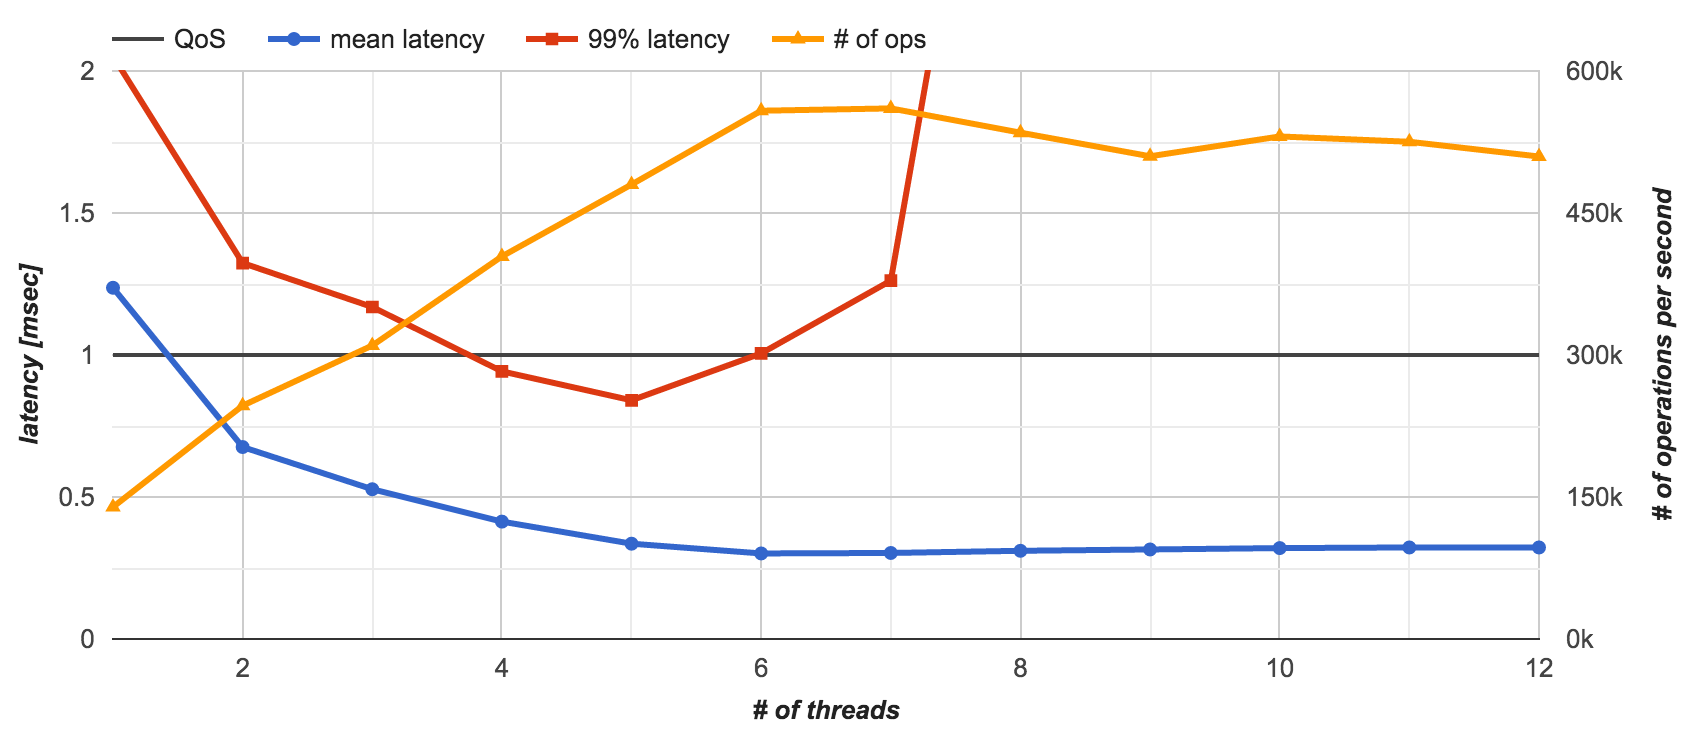
\includegraphics[width=\textwidth]{./res2/m_threads_latency.png}
    \caption{Memcached Threads: Latency \& Throughput vs Number of Threads}
    \label{fig:m_threads_latency.png}
\end{figure}

Firstly, mean latency (\textit{blue}) decreases as the number of threads increases from 1 to 6 where it reaches a minimum of 0.301ms. As the numbr of threads grows beyond 6, the mean latency increases at a slow pace.

Secondly, 99th percentile latency (\textit{red}) starts at 2.05ms, above the required QoS. As the number of threads increases, the 99th percentile latency drops sharply. With 4 to 6 threads, the 99th percentile latency satisfies the QoS with a minimum of 0.84ms reached at 5 threads. Beyond 6 threads, the 99th percentile latency rises sharply beyond the required QoS.

Thirdly, the number of operations per second (\textit{yellow}), increases linearly with the number of threads up until 6 threads where it reaches a maximum of 558k requests per second. A further increase in the number of threads results in a decrease of the number of operations per second.

Overall, QoS constraints are only achieved with 4 to 6 threads. We can attribute this effect to the multi threaded design of Memcached. With 3 threads or less, the load exerted by the clients cannot be processed quickly resulting in requests being queued up. This leads to an increased 99th percentile latency. With a sufficient number of threads to process the load effectively, a CPU core is able to service the requests sooner and therefore reduce the 99th percentile latency while also increasing the total number of operations.

With more than 6 threads, the kernel is forced to schedule multiple threads on the same core. This effect is described as `load imbalance' by Leverich \& Kozyrakis. With more than 1 Memcached thread executing on a single core, it is reasonable to expect the throughput to decrease, as opposed to only 1 Memcached thread per each core, due to context switching.

Overall, the best performance in terms of maximizing throughput and minimizing latency is provided by as many threads as CPU cores, in our case 6 threads. However, this is not in fact the minimum 99th percentile latency achieved in the benchmark - at 5 threads we obtain 99th percentile latency of 0.84ms with 480k requests per second.


\subsection{CPU Utilization}

Figure \ref{fig:m_threads_cpu} provides the \textit{mpstat} category breakdown of the CPU utilization of Memcached during the benchmark. Note that unattributed utilization accounts for idle time.

\begin{figure}[h]
    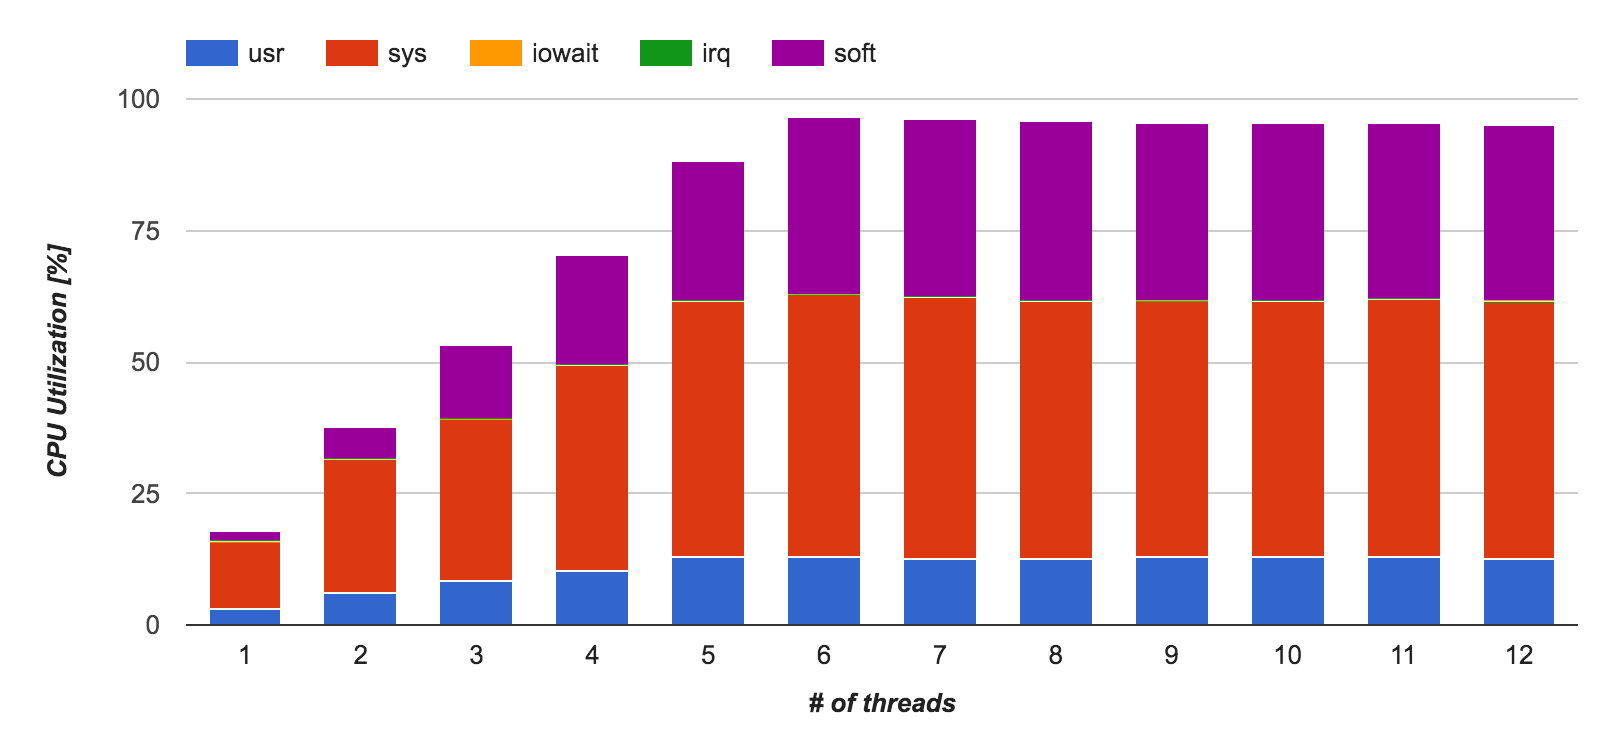
\includegraphics[width=\textwidth]{./res2/m_threads_cpu.png}
    \caption{Memcached CPU Utilization with Multiple Threads}
    \label{fig:m_threads_cpu}
\end{figure}

Firstly, Memcached CPU usage (\textit{usr}) increases linearly with the number of instances up to 6 threads and accounts for 12.7\%. With more than 6 threads, the Memcached CPU usage remains constant. This is reasonable as Memcached itself is not CPU intensive, however, a larger number of threads will require more CPU to operate effectively. Consequently, with more than 6 threads, context switching occurs due to insufficient number of CPU cores to monopolize a given core and therefore the CPU usage remains constant.

Secondly, kernel utilization increases with the number of threads up to 6 threads at which point it stabilizes and accounts for 50\%. A further increase in the number of threads does not result in increased utilization. It is reasonable to expect a large kernel CPU utilization as it is responsible for receiving and sending of network requests and memcached is a network bound application \cite{belay2014ix}.

Thirdly, similarly to kernel CPU usage, CPU utilization for software interrupts (\textit{soft}) increases with the number of threads. At 6 threads, it accounts for 33.7\%. The increase in the time spent processing software interrupts is due to overall increase in throughput as requests are processed faster. An increase in the number of requests per second directly results in an increase in the number of software interrupts received and issued by \textit{libevent}.

Finally, we observe no disk I/O wait as Memcached is an in memory object cache and therefore does not access the hard drive unless the memory is exhausted and swapping to disk is triggered. Additionally, hardware interrupt servicing \textit{irq} only accounts for 0.01\% as batching in the NIC is enabled.


\subsection{Thread Evaluation}
Increasing the number of Memcached threads results in increased throughput and decreased latency. The best performing configuration observed is with as many threads as there are CPU cores. The direct cost of increased number of threads is CPU utilization.

% ________________________________________________________

\section{Thread pinning}
\label{sec:thread-pinning}
Thread pinning is the process of assigning a \textit{set\_irq\_affinity} to each individual thread. As suggested by Leverich and Kozyrakis, "pinning memcached threads to distinct cores greatly improves load balance, consequently improving tail latency." \cite{leverich2014reconciling} and therefore the reasonable next step in optimizing memcached performance is to attempt thread pinning and analyse the results obtained.

By default, when a new process is started, its affinity is set to all available CPUs. We can discover the affinity of a given process through the following command where \textit{pid} is the process identifier.

\begin{lstlisting}
    taskset -p <pid>
\end{lstlisting}


"A Memcache instance started with n threads will spawn n + 1 threads of which the first n are worker threads and the last is a maintenance thread used for hash table expansion under high load factor." \cite{solarflarememcached}. We can discover memcached threads used for request processing using the following command where \textit{tid} is the thread id discovered previously \cite{solarflarememcached}.
\begin{lstlisting}
    ps -p <memcache-pid> -o tid= -L | sort -n | tail -n +2 | head -n -1
\end{lstlisting}

For this benchmark, the previous configuration with 6 threads will be used.

\subsection{Latency \& Throughput vs Threads}

Figure \ref{fig:m_pinning_latency} presents a comparison of Memcached with pinned threads against unpinned threads.

\begin{figure}[h]
    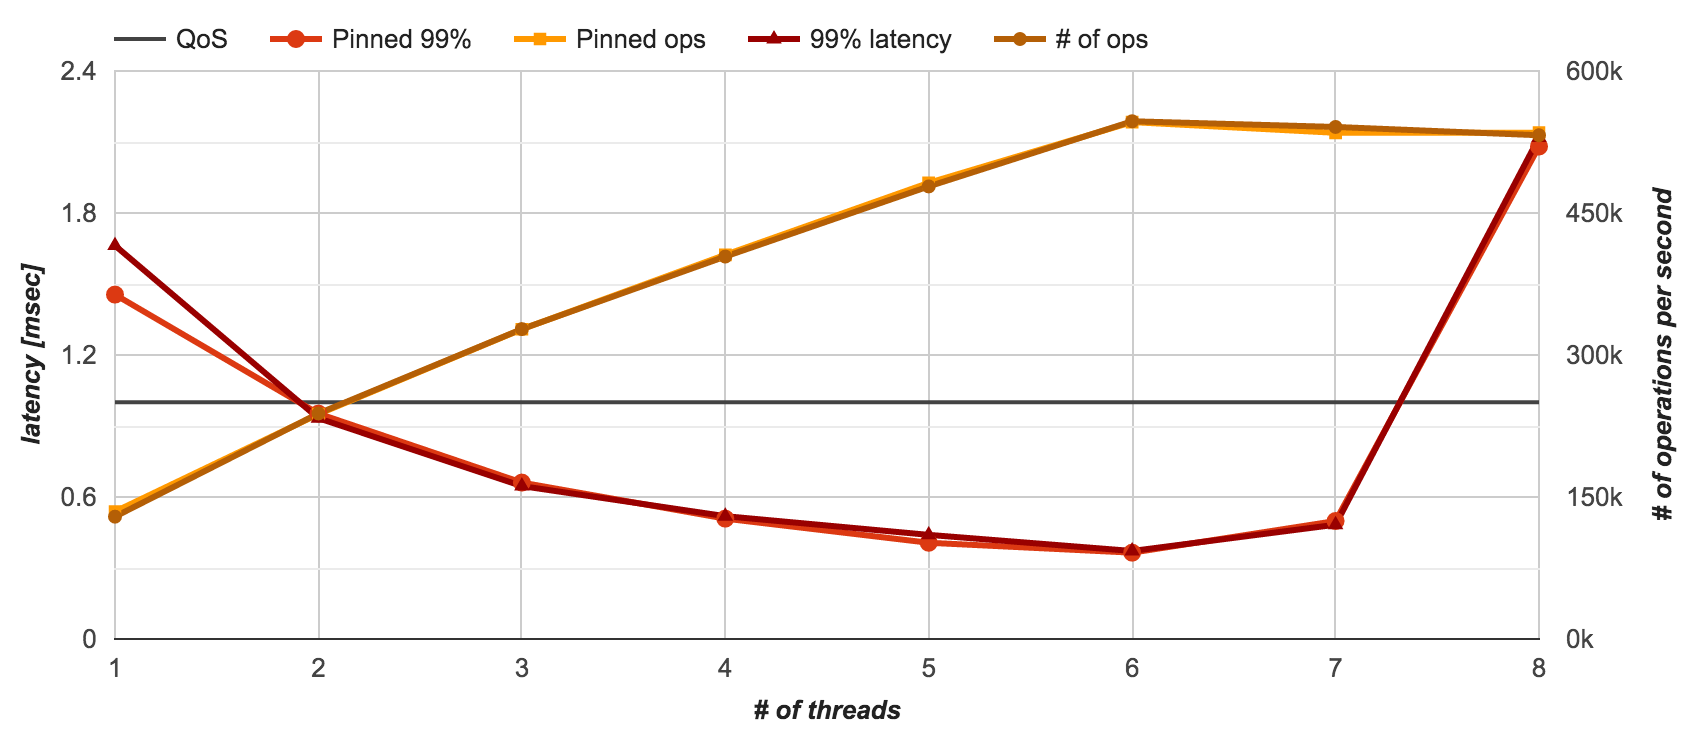
\includegraphics[width=\textwidth]{./res2/m_pinning_latency.png}
    \caption{Memcached Latency \& Throughput vs Threads: Comparison of pinned threads (labeled: \textit{Pin}) vs unpinned threads}
    \label{fig:m_pinning_latency}
\end{figure}

Overall, we can observe that there is very little change in all of the results observed. Mean latency remains the same, 99th percentile latency only differs slightly in it's minimum value at 5 threads and the number of operations per second remains the same. Overall, we find that in our benchmarks thread pinning does not affect performance significantly. This is contrary to results reported by Leverich and Kozyrakis \cite{leverich2014reconciling}. According to their research, thread pinning results in improved load balance and a result decreases 99th percentile latency. This in turn results in increased throughput.

\subsection{CPU Utilization}

Figure \ref{fig:m_pinning_cpu} presents the CPU Usage with Memcached threads pinned.

\begin{figure}[h]
    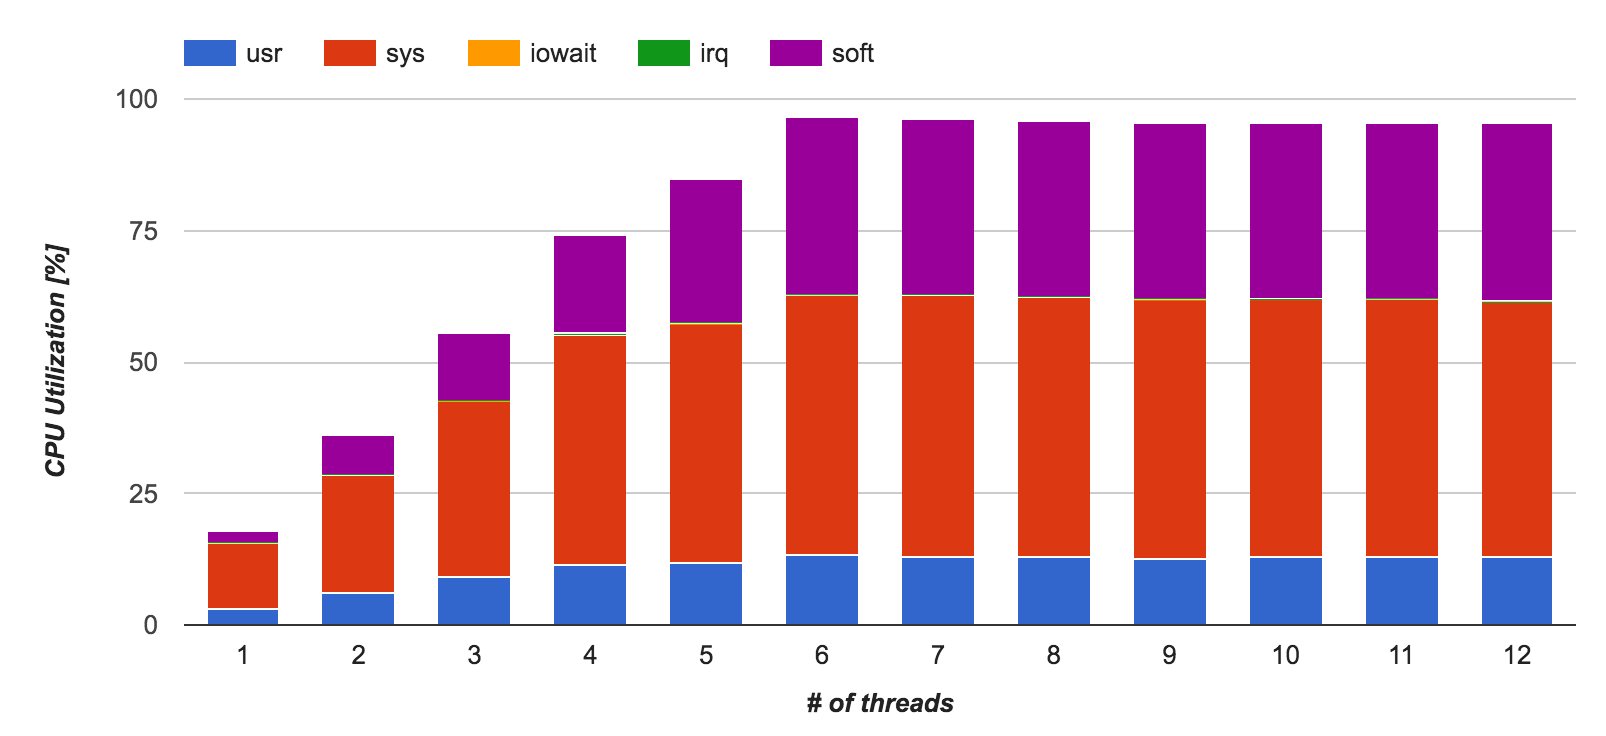
\includegraphics[width=\textwidth]{./res2/m_pinning_cpu.png}
    \caption{Pinned Memcached CPU Utilization}
    \label{fig:m_pinning_cpu}
\end{figure}

The CPU Utilization of pinned threads is nearly identical to unpinned threads presented in Figure \ref{fig:m_threads_cpu}.

\subsection{Thread Pinning Conclusion}

In our benchmarks, we have not been able to achieve the significant improvements in both latency and throughput suggested to be gained by thread pinning. This is likely due to differences in hardware as Leverich and Kozyrakis \cite{leverich2014reconciling} perform benchmarks on a significantly more performant hardware as well as running on a slightly older version of memcached.


\section{Group Size}
Memcached provides a configuration option \textit{-R} to set the group size used inside memcached. The group size defines the ``Maximum number of requests per event, limits the number of requests process for a given connection to prevent starvation (default: 20)'' \cite{interactive2006memcached}. This in effect means the number of requests that will be processed from a single connection before memcached switches to a different connection to achieve a fair policy.

In order to benchmark the effects of an increased group size, we consider a benchmark scenario where the group size is progressively increased while maintaining a consistent load on the cache. The load used will be the one explored in Section \ref{sec:thread-pinning} - Thread Pinning. All clients will be setup with 2 threads and 9 connections each which corresponds to the best performance under QoS so far. The memcached server will be setup with the \textit{-R} flag set to 20 initially and increased by 20 for each iteration until a maximum (enforced by memcached) of 320 is reached.

\begin{figure}[h]
    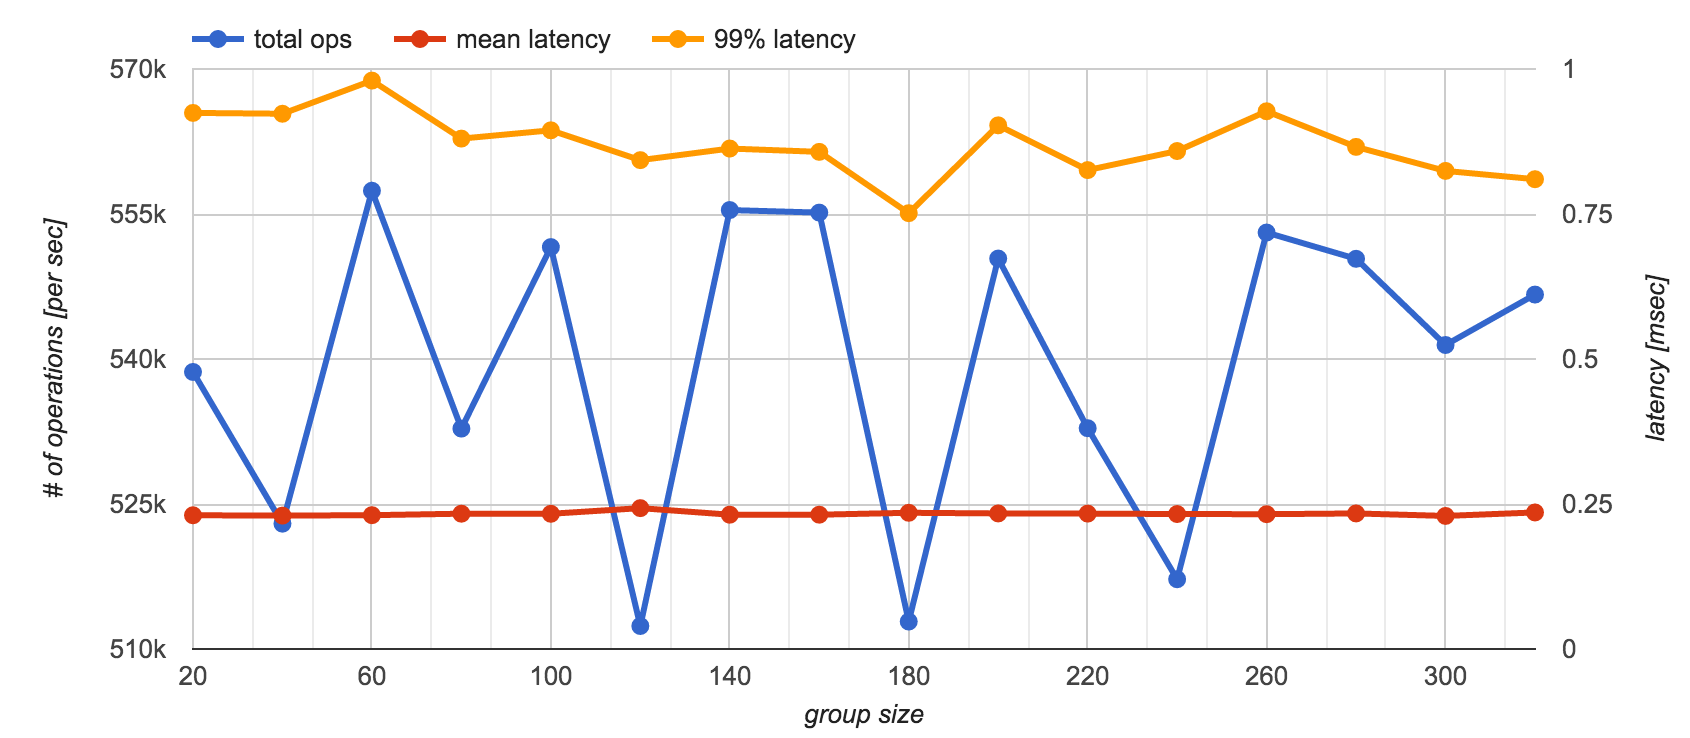
\includegraphics[width=\textwidth]{./res/5_memcached_group_size.png}
    \caption{Memcached Latency, 99th percentile latency and throughput against group size}
    \label{fig:memcached_group_size}
\end{figure}

Figure \ref{fig:memcached_group_size} shows the relationship between throughput, mean latency and 99th percentile latency.

Firstly, we can observe that the throughput achieved fluctuates heavily around 540k requests per second. Secondly, the mean latency remains constant as the group size is increased. Finally, the 99th percentile latency experiences a decreasing trend as group size is increased while staying under the required QoS constraints of 1ms.

By setting \textit{group size} to 320, we have been able to reduce both 99th percentile latency as well as increase the total throughput from 520k to 540k requests per second. Additionally, we have been able to show that the context switching required to achieve a fairness policy of processing only 20 requests from a single connection caused a decrease in performance. Similar results have been obtained by Blake and Saidi \cite{blake54does}. On the other hand, the results observed are dependent on the distributed system model and the expected request rate. In a production environment, benchmarking of a particular workload would show the best configuration in respect to group size.

\section{Receive \& Transmit Queues fixing}
TODO: Haven't been able to obtain any improvements in terms of performance (both throughput and latency), not sure if the topic should still be discussed in detail.


\section{Multiple Memcached Processes}

In this section, we will examine the impact multiple memcached processed have on the overall performance of the caches as a whole. In some applications, it is important to be able to partition the system in such a way systems interact with different instances of memcached. Additionally, this information will also serve as a useful benchmark comparison for Redis performance.